\documentclass{standalone}
\usepackage{graphicx}	
\usepackage{amssymb, amsmath, amsthm}
\usepackage{color}

\usepackage{tikz}
\usetikzlibrary{math, calc, decorations.pathreplacing}

\definecolor{light}{RGB}{220, 188, 188}
\definecolor{mid}{RGB}{185, 124, 124}
\definecolor{dark}{RGB}{143, 39, 39}
\definecolor{highlight}{RGB}{180, 31, 180}
\definecolor{gray10}{gray}{0.1}
\definecolor{gray20}{gray}{0.2}
\definecolor{gray30}{gray}{0.3}
\definecolor{gray40}{gray}{0.4}
\definecolor{gray60}{gray}{0.6}
\definecolor{gray70}{gray}{0.7}
\definecolor{gray80}{gray}{0.8}
\definecolor{gray90}{gray}{0.9}
\definecolor{gray95}{gray}{0.95}

% #1: x0
% #2: y0
% #3: R
\newcommand{\randpoints}[3]{
  ({#1 + (1 + 0.2 * rand) * #3 * (-1)},      {#2 + (1 + 0.2 * rand) * #3 * (0)})
  ({#1 + (1 + 0.2 * rand) * #3 * (-0.7071)}, {#2 + (1 + 0.2 * rand) * #3 * (+0.7071)})
  ({#1 + (1 + 0.2 * rand) * #3 * (0)},       {#2 + (1 + 0.2 * rand) * #3 * (+1)})
  ({#1 + (1 + 0.2 * rand) * #3 * (+0.7071)}, {#2 + (1 + 0.2 * rand) * #3 * (+0.7071)})
  ({#1 + (1 + 0.2 * rand) * #3 * (+1)},      {#2 + (1 + 0.2 * rand) * #3 * (0)})
  ({#1 + (1 + 0.2 * rand) * #3 * (+0.7071)}, {#2 + (1 + 0.2 * rand) * #3 * (-0.7071)})
  ({#1 + (1 + 0.2 * rand) * #3 * (0)},       {#2 + (1 + 0.2 * rand) * #3 * (-1)})
  ({#1 + (1 + 0.2 * rand) * #3 * (-0.7071)}, {#2 + (1 + 0.2 * rand) * #3 * (-0.7071)})
}

\begin{document}

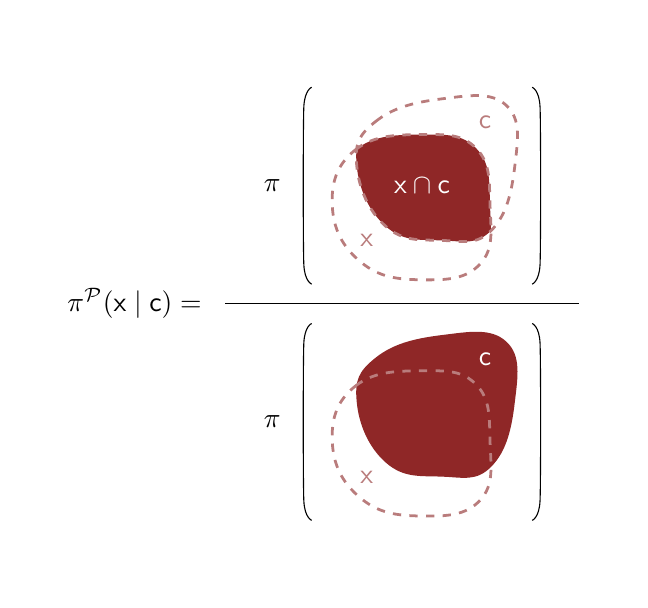
\begin{tikzpicture}[scale=1]
  \draw[white] (2, -3.5) rectangle (9.5, 3.5);
  
  \node at (3.35, 0) { $\pi^{\mathcal{P}}( \mathsf{x} \mid \mathsf{c} ) =$ };

  \begin{scope}[shift={(7, 1.5)}]  
    \node at (-1.9, 0) { $\pi$ };
    \draw plot [smooth, tension=0.35] coordinates { (-1.4, -1.25) (-1.5, -1) (-1.5, 1) (-1.4, 1.25) };
    \draw plot [smooth, tension=0.35] coordinates { (+1.4, -1.25) (+1.5, -1) (+1.5, 1) (+1.4, 1.25) };
  
    \begin{scope}
      \pgfmathsetseed{1}
      \clip plot [smooth cycle, tension=0.75] coordinates { \randpoints{0}{-0.25}{1} } -- cycle;
      \pgfmathsetseed{2}
      \fill[dark, dashed, line width=1] 
        plot [smooth cycle, tension=0.75] coordinates { \randpoints{0.25}{0.25}{1} } -- cycle;
    \end{scope}

    \pgfmathsetseed{1}
    \draw[mid, dashed, line width=1] 
      plot [smooth cycle, tension=0.75] coordinates { \randpoints{0}{-0.25}{1} } -- cycle;
    
    \pgfmathsetseed{2}
    \draw[mid, dashed, line width=1] 
      plot [smooth cycle, tension=0.75] coordinates { \randpoints{0.25}{0.25}{1} } -- cycle;
    
    \node[mid] at (-0.7, -0.7) { $\mathsf{x}$ };
    \node[mid] at (+0.8, +0.8) { $\mathsf{c}$ };
    \node[white] at (0, 0) { $\mathsf{x} \cap \mathsf{c}$ };
  \end{scope}
  
  \draw (4.5, 0) -- (9, 0);
  
  \begin{scope}[shift={(7, -1.5)}]
    \node at (-1.9, 0) { $\pi$ };
    \draw plot [smooth, tension=0.35] coordinates { (-1.4, -1.25) (-1.5, -1) (-1.5, 1) (-1.4, 1.25) };
    \draw plot [smooth, tension=0.35] coordinates { (+1.4, -1.25) (+1.5, -1) (+1.5, 1) (+1.4, 1.25) };
    
    \pgfmathsetseed{2}
    \fill[dark, dashed, line width=1] 
      plot [smooth cycle, tension=0.75] coordinates { \randpoints{0.25}{0.25}{1} } -- cycle;
    
    \pgfmathsetseed{1}
    \draw[mid, dashed, line width=1] 
      plot [smooth cycle, tension=0.75] coordinates { \randpoints{0}{-0.25}{1} } -- cycle;
    
    \node[mid] at (-0.7, -0.7) { $\mathsf{x}$ };
    \node[white] at (+0.8, +0.8) { $\mathsf{c}$ };
    
  \end{scope}
  
\end{tikzpicture}

\end{document}  